\documentclass[oneside, 11pt]{article}

\usepackage[T1]{fontenc}
\usepackage[utf8]{inputenc}
\usepackage[english]{babel}

\usepackage{fouriernc}
\usepackage[detect-all, binary-units, separate-uncertainty=true,
            per-mode=symbol, retain-explicit-plus, retain-unity-mantissa=false]{siunitx}

\usepackage{setspace}
\setstretch{1.2}

\setlength{\parskip}{\smallskipamount}
\setlength{\parindent}{0pt}

\usepackage[headheight=14pt]{geometry}
\geometry{marginparwidth=0.5cm, verbose, a4paper, tmargin=3cm, bmargin=3cm,
          lmargin=2cm, rmargin=2cm}

\usepackage{float}

\usepackage[fleqn]{amsmath}
\numberwithin{equation}{section}
\numberwithin{figure}{section}

\usepackage{graphicx}
\graphicspath{{images/}{../../../images/}}

\usepackage{tikz}
\usetikzlibrary{shapes}
\usetikzlibrary{plotmarks}

\newcounter{Exercise}
\setcounter{Exercise}{1}
\usepackage{xcolor}
\definecolor{shadecolor}{gray}{0.9}
\usepackage{framed}
\usepackage{caption}

\usepackage{url}


\usepackage{fancyhdr}
\pagestyle{fancy}
\fancyhf{}
\rhead{\thepage}
\renewcommand{\footrulewidth}{0pt}
\renewcommand{\headrulewidth}{0pt}

\fancypagestyle{firststyle}
{
    \fancyhf{}
    \rhead{\thepage}
    \cfoot{
\includegraphics[height=30pt]{HiSPARClogo}}
    \rfoot{
\includegraphics[height=25pt]{CCbysa}}
    \lfoot{
\includegraphics[height=30pt]{NIKHEFlogo}}
    \renewcommand{\footskip}{50pt}
    \renewcommand{\footrulewidth}{0.1pt}
    \renewcommand{\headrulewidth}{0pt}
}

\newcommand{\figref}[1]{Figuur~\ref{#1}}

\newcommand{\hisparc}{\textsmaller{HiSPARC}\xspace}
\newcommand{\kascade}{\textsmaller{KASCADE}\xspace}
\newcommand{\sapphire}{\textsmaller{SAPPHiRE}\xspace}
\newcommand{\jsparc}{\textsmaller{jSparc}\xspace}
\newcommand{\hdf}{\textsmaller{HDF5}\xspace}
\newcommand{\aires}{\textsmaller{AIRES}\xspace}
\newcommand{\csv}{\textsmaller{CSV}\xspace}
\newcommand{\python}{\textsmaller{PYTHON}\xspace}
\newcommand{\corsika}{\textsmaller{CORSIKA}\xspace}
\newcommand{\labview}{\textsmaller{LabVIEW}\xspace}
\newcommand{\daq}{\textsmaller{DAQ}\xspace}
\newcommand{\adc}{\textsmaller{ADC}\xspace}
\newcommand{\hi}{\textsc{h i}\xspace}
\newcommand{\hii}{\textsc{h ii}\xspace}
\newcommand{\mip}{\textsmaller{MIP}\xspace}
\newcommand{\hisparcii}{\textsmaller{HiSPARC II}\xspace}
\newcommand{\hisparciii}{\textsmaller{HiSPARC III}\xspace}

\DeclareSIUnit{\electronvolt}{\ensuremath{\mathrm{e\!\!\:V}}}

\DeclareSIUnit{\unitsigma}{\ensuremath{\sigma}}
\DeclareSIUnit{\mip}{\textsmaller{MIP}}
\DeclareSIUnit{\adc}{\textsmaller{ADC}}

\DeclareSIUnit{\gauss}{G}
\DeclareSIUnit{\parsec}{pc}
\DeclareSIUnit{\year}{yr}



\begin{document}

\title{Botsingen}
\author{N.G. Schultheiss}
\date{}

\maketitle
\thispagestyle{firststyle}

\section{Inleiding}

In de natuur oefenen voorwerpen krachten op elkaar uit. Dit kan bijvoorbeeld
doordat twee voorwerpen met elkaar botsen. We kunnen hier denken aan
grote samengestelde voorwerpen voorwerpen, maar ook aan kleine voorwerpen.
Een scheikundige reactie is misschien wel te beschouwen als een soort
botsing van atomen (of moleculen) waardoor een (ander) molecule onstaat.

Botsingen zijn op twee manieren te beschouwen, elastische botsingen
en niet-elastische botsingen. Een scheikundige reactie is te beschouwen
als een niet-elastische botsing. Kernreacties zijn ook te beschouwen
als niet-elastische botsingen.


\section{Behoudswetten}

Bij botsingen bestuderen we systemen van verschillende objecten. We
kunnen bij\-voorbeeld denken aan een botsing van een scooterrijder
met een vuilnisbak. Dit is een scooterrijder/vuilnisbak systeem te
noemen. Volgens de derde wet van Newton ($\mathbf{F}_{actie}=-\mathbf{F}_{reactie}$)
\footnote{Ik gebruik voor de vector van de kracht ``$\mathbf{F}$'', de grootte
wordt geschreven met ``$F$''.
} oefenen beide objecten in het systeem op ieder moment een even grote
maar tegengestelde kracht uit
\footnote{Let op: Dit is een ander situatie dan een object waarbij alle
krachten die op dat object werken in evenwicht zijn. Dit laatste is een
bijzonder geval van de tweede wet Newton.}. Voor en na de botsing is deze kracht 0N. Gedurende de botsing, die
voor beide objecten even lang duurt, zijn er twee even grote en tegengestelde
krachten. Als voorwerp I gedurende de botsing vertraagt, versnelt
voorwerp II. We kunnen deze (eenparig) versnelde bewegingen dus nader
bestuderen met de tweede wet van Newton:

\begin{equation}
\mathbf{F}=m\mathbf{a}\Longleftrightarrow
\end{equation}


\begin{equation}
\mathbf{F}=m\frac{\Delta\mathbf{v}}{\Delta t}\Longleftrightarrow
\end{equation}


\begin{equation}
\mathbf{F}\Delta t=m\Delta\mathbf{v}=\Delta\mathbf{p}
\end{equation}


Deze laatste schrijfwijze komt bij botsingen veel voor en wordt ook
wel de impulsverandering genoemd. Omdat de krachten tegengesteld zijn
en de duur hetzelfde is, neemt de impuls in het geval van de scooterrijder
net zo veel af, als de impuls van de vuilnisbak toeneemt. We kunnen
dus zeggen dat de som van de impulsen van alle objecten in het systeem
voor en na de botsing hetzelfde is. Dit noemt men ook wel de wet van
behoud van impuls. 

\begin{equation}
\sum\mathbf{p}=constant
\end{equation}


In de klassieke natuurkunde berekent men de impuls van een object
overigens vaak met:

\begin{equation}
\mathbf{p}=m\mathbf{v}
\end{equation}


Naast de wet van behoud van impuls kennen we de wet van behoud van
energie. Uiteraard heb je hier wel eens van gehoord. Voor de volledigheid
volgt toch een korte wiskundige bespreking van deze wet voor botsingen.
We gaan eerst uit van een elastische botsing. Nu zal er geen energie
worden omgezet in bijvoorbeeld warmte.

We hebben al gezien dat een botsing voor beide objecten even lang duurt.
Uiteraard verplaatst het punt waar beide objecten elkaar raken ook even
veel. De krachten die door de objecten op elkaar in dit punt worden
uitgeoefend zijn nu ook weer tegengesteld en even groot. De
energieoverdracht van object \emph{I} naar de object \emph{II} is in dit
geval met de arbeid \footnote{Pizzakoeriers kunnen als scooterrijder
natuurlijk best arbeid verrichten. In het geval van de natuurkunde is
het echter zo dat alleen krachten arbeid verrichten.} uit te rekenen.

\begin{equation}
W=\mathbf{F}.\mathbf{s}\Longrightarrow
\end{equation}


\begin{equation}
\left\{ \begin{array}{c}
W_{I}=\mathbf{F}_{I}.\mathbf{s}\\
W_{II}=\mathbf{F}_{II}.\mathbf{s}\\
-\mathbf{F}_{I}=\mathbf{F}_{II}
\end{array}\right\} \Longrightarrow
\end{equation}


\begin{equation}
-W_{I}=W_{II}
\end{equation}


Omdat object \emph{I}, via arbeid, net zo veel energie levert als
object \emph{II} ontvangt, kunnen we zeggen dat de som van de energie
van object \emph{I} en object \emph{II} gelijk blijft. De wet van
behoud van energie klopt dus voor elastische botsingen.

\begin{equation}
\sum E=constant
\end{equation}


Laten we eens zien of hier een elastische botsing mee te berekenen
is. We nemen een scooterrijder (object \emph{I}) van 60kg. Deze raakt
een stilstaande vuilnisbak (object \emph{II}) van 30kg met een snelheid
van 10m/s. Dit is ook te schrijven als:\\
\\
Gegeven voor de botsing: 

$v_{I}=10${[}m/s{]}

$m_{I}=60${[}kg{]}

$v_{II}=0${[}m/s{]}

$m_{II}=30${[}kg{]}\\
\\
Gevraagd: De snelheden na de botsing.\\
\\
Oplossing:

Energie tijdens de botsing: $E_{systeem}=\frac{1}{2}m_{I}(v_{I})^{2}+\frac{1}{2}m_{II}(v_{II})^{2}$

Of voor de botsing: $E_{systeem}=\frac{1}{2}60${[}kg{]}$(10${[}m/s{]}$)^{2}=3000${[}J{]}

Impuls tijdens de botsing: $p=m_{I}v_{I}+m_{II}v_{II}$

Of voor de botsing: $p=60${[}kg{]}$10${[}m/s{]}$=600${[}kgm/s{]}\\


Impuls na de botsing: $60${[}kg{]}$v_{I}+30${[}kg{]}$v_{II}=600${[}kgm/s{]}$\Longleftrightarrow$$v_{II}=20${[}kgm/s{]}$-2v_{I}$

Substitutie geeft: $E_{systeem}=\frac{1}{2}60\mathrm{[kg]}(v_{I})^{2}+\frac{1}{2}30\mathrm{[kg]}(20${[}kgm/s{]}$-2v_{I})^{2}=3000$J

Uitwerken geeft: $v_{I}=10${[}m/s{]} en $v_{I}=3,3${[}m/s{]}

Deze kwadratische vergelijking heeft dus twee oplossingen, één voor
de botsing en één na de botsing.

Invullen in $v_{II}=20${[}kgm/s{]}$-2v_{I}$ geeft de bijbehorende
snelheden van object \emph{II}: $v_{II}=0${[}m/s{]} en $v_{II}=13${[}m/s{]}.

Na de botsing gaat de scooterrijder dus 3,3{[}m/s{]} en de vuilnisbak
13{[}m/s{]}.

Stel dat de scooterrijder stil ligt na de botsing. Kunnen we dan uitrekenen
hoeveel energie er in warmte is omgezet? Uiteraard blijft de wet van
behoud van impuls gelden. Omdat de scooterrijder stil ligt, zit alle
impuls in de vuilnisbak. Omdat de massa van de vuilnisbak de helft
van de massa van de scooterrijder is, wordt de snelheid tweemaal zo
groot, of 20{[}m/s{]}. De energie van de vuilnisbak is dan 6000{[}J{]}.
Dit is twee maal zo veel als voor de botsing. We kunnen dus alleen
maar de conclusie trekken dat dit niet kan. Het scooterrijder/vuilnisbak
systeem heeft namelijk te weinig energie.

\paragraph*{Opdracht 1:} \emph{Bereken hoeveel energie er (bijvoorbeeld
in warmte) wordt omgezet als de scooterrijder na de bot\-sing een
snelheid van 5,0{[}m/s{]} heeft.}

\paragraph*{Opdracht 2:} \emph{Bereken hoeveel energie er (bijvoorbeeld
in warmte of een soort ``plak-energie'') wordt omgezet als de
scooterrijder en de vuilnisbak aan elkaar plakken.}


\section{Schuine botsingen}

In het vorige hoofdstuk hebben we gezien hoe scooterrijders met vuilnisbakken
botsen. Impliciet is hier aangenomen dat het centrale botsingen betreft.
In de praktijk is dit meestal niet het geval.

Om schuine botsingen te bespreken, kijken we naar eenvoudig snookeren.
Er wordt dus zonder effect gespeeld. De truc om een te potten bal
in een pocket te schieten is om over de bal naar de pocket te kijken.
De speelbal (wit) moet de te potten bal (zwart) dan precies in het
verlengde raken. De lijn door de middelpunten van de twee ballen wijst
dan naar de pot waar de te potten bal in wordt geschoten.

\begin{figure}[H]
\noindent \begin{centering}
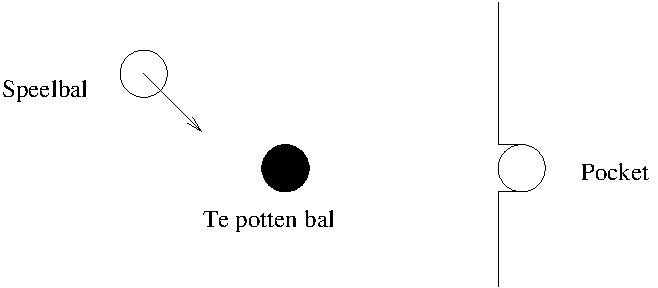
\includegraphics[scale=0.75]{snooker1}
\par\end{centering}

\caption{Voor de botsing}
\end{figure}


De impulsvector van de speelbal is te onbinden in een $\mathbf{p_{\mathrm{\mathit{x}}}}$
en een $\mathbf{p_{y}}$ component. Het assenstelsel zit nu aan de
snookertafel vast. 

We nemen een nieuwe assenstelsel dat met de y-as aan de speelbal vastzit.

\begin{figure}[H]
\noindent \begin{centering}
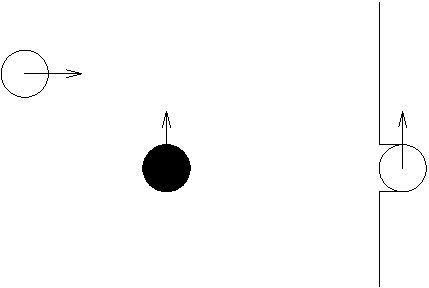
\includegraphics[scale=0.75]{snooker2}
\par\end{centering}

\caption{Botsing 1}
\end{figure}


De pocket en de te potten bal bewegen in dit assenstelsel in de richting
van de positieve y-as. De speelbal beweegt in de richting van de positieve
x-as en maakt nu een centrale botsing met de te potten bal. Beide
ballen hebben dezelfde massa.

\paragraph*{Opdracht 3:} \emph{Toon aan dat de speelbal in dit assenstelsel alle impuls
aan de te potten bal overdraagt.}

De te potten bal krijgt nu twee componenten van impuls, de speelbal
ligt stil.

\begin{figure}[H]
\noindent \begin{centering}
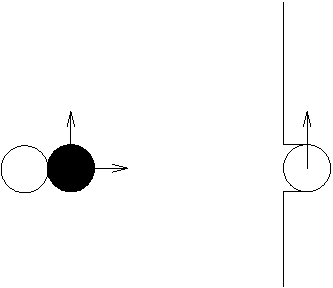
\includegraphics[scale=0.75]{snooker3}
\par\end{centering}

\caption{Botsing 2}
\end{figure}


We maken het assenstelsel nu weer aan de tafel vast. De speelbal beweegt
in negatieve y-richting, de te potten bal beweegt in de positieve
x-richting en de pocket blijft uiteraard in rust.

\begin{figure}[H]
\noindent \begin{centering}
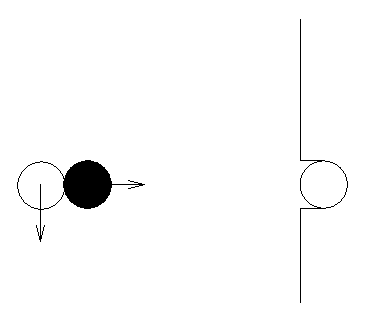
\includegraphics[scale=0.75]{snooker4}
\par\end{centering}

\caption{Na de botsing}
\end{figure}

Het snookerprobleem is dus oplosbaar door twee maal van assenstelsel
te veranderen.

\end{document}
